\documentclass[
	9pt, % Set the default font size, options include: 8pt, 9pt, 10pt, 11pt, 12pt, 14pt, 17pt, 20pt
	t, % Uncomment to vertically align all slide content to the top of the slide, rather than the default centered
	%aspectratio=169, % Uncomment to set the aspect ratio to a 16:9 ratio which matches the aspect ratio of 1080p and 4K screens and projectors
]{beamer}

\graphicspath{{Images/}{./}} % Specifies where to look for included images (trailing slash required)

\usepackage{booktabs} % Allows the use of \toprule, \midrule and \bottomrule for better rules in tables
\usepackage{graphicx}
\usepackage{caption}
\usepackage{subcaption}
\usepackage{hyperref}
\usepackage[english,brazil]{babel}
\usepackage{fontawesome5}
\usepackage{listings}
\usepackage{minted}
\usepackage{xcolor}
% \usepackage{graphicx}
% \usepackage{animate}
\RequirePackage[backend=biber,
style=ieee,
citestyle=authoryear,
]{biblatex}

% Define a custom command for an icon link
\newcommand{\iconLink}[2]{\href{#1}{\faLink \hspace{0.2em} {#2}}}
\newcommand{\yellowbox}[1]{\colorbox{yellow!75}{#1}}
\definecolor{darkgreen}{rgb}{0,0.5,0}

% Definindo um estilo para o destaque
%----------------------------------------------------------------------------------------
%	SELECT LAYOUT THEME
%----------------------------------------------------------------------------------------
\usetheme{Madrid}

%----------------------------------------------------------------------------------------
%	SELECT COLOR THEME
%----------------------------------------------------------------------------------------

% Beamer comes with a number of color themes that can be applied to any layout theme to change its colors. Uncomment each of these in turn to see how they change the colors of your selected layout theme.

%\usecolortheme{albatross}
%\usecolortheme{beaver}
%\usecolortheme{beetle}
% \usecolortheme{crane}
%\usecolortheme{dolphin}
%\usecolortheme{dove}
%\usecolortheme{fly}
%\usecolortheme{lily}
%\usecolortheme{monarca}
%\usecolortheme{seagull}
%\usecolortheme{seahorse}
%\usecolortheme{spruce}
%\usecolortheme{whale}
%\usecolortheme{wolverine}

%----------------------------------------------------------------------------------------
%	SELECT FONT THEME & FONTS
%----------------------------------------------------------------------------------------
\usefonttheme{default} % Typeset using the default sans serif font

%------------------------------------------------

\usepackage{palatino} % Use the Palatino font for serif text
\usepackage[default]{lato} % Use the Lato font for sans serif text

%----------------------------------------------------------------------------------------
%	SELECT INNER THEME
%----------------------------------------------------------------------------------------
\useinnertheme{rectangles}

%----------------------------------------------------------------------------------------
%	SELECT OUTER THEME
%----------------------------------------------------------------------------------------

% Outer themes change the overall layout of slides, such as: header and footer lines, sidebars and slide titles. Uncomment each theme in turn to see what changes it makes to your presentation.

%\useoutertheme{default}
%\useoutertheme{infolines}
%\useoutertheme{miniframes}
%\useoutertheme{smoothbars}
%\useoutertheme{sidebar}
%\useoutertheme{split}
%\useoutertheme{shadow}
%\useoutertheme{tree}
%\useoutertheme{smoothtree}

%\setbeamertemplate{footline} % Uncomment this line to remove the footer line in all slides
%\setbeamertemplate{footline}[page number] % Uncomment this line to replace the footer line in all slides with a simple slide count

%\setbeamertemplate{navigation symbols}{} % Uncomment this line to remove the navigation symbols from the bottom of all slides

% \bibliography{references} % Specifies the bibliography file to include publications
% \bibliographystyle{apalike} % Specifies the bibliography style
\addbibresource{references.bib}

%----------------------------------------------------------------------------------------
%	PRESENTATION INFORMATION
%----------------------------------------------------------------------------------------

\title[DesWebII]{Desenvolvimento Web II} % The short title in the optional parameter appears at the bottom of every slide, the full title in the main parameter is only on the title page
\subtitle{Aula 07 - Uso de Mensageria e Filas de Mensagens} % Presentation subtitle, remove this command if a subtitle isn't required
\author[Fabricio Bizotto]{Prof. Fabricio Bizotto} % Presenter name(s), the optional parameter can contain a shortened version to appear on the bottom of every slide, while the main parameter will appear on the title slide
\institute[IFC]{Instituto Federal Catarinense \\ \smallskip \textit{fabricio.bizotto@ifc.edu.br}} % Your institution, the optional parameter can be used for the institution shorthand and will appear on the bottom of every slide after author names, while the required parameter is used on the title slide and can include your email address or additional information on separate lines
\date[\today]{Ciência da Computação \\ \today} % Presentation date or conference/meeting name, the optional parameter can contain a shortened version to appear on the bottom of every slide, while the required parameter value is output to the title slide

%----------------------------------------------------------------------------------------
\begin{document}

%----------------------------------------------------------------------------------------
%	TITLE SLIDE
%----------------------------------------------------------------------------------------

\begin{frame}
	\titlepage % Output the title slide, automatically created using the text entered in the PRESENTATION INFORMATION block above
\end{frame}

%----------------------------------------------------------------------------------------
%	TABLE OF CONTENTS SLIDE
%----------------------------------------------------------------------------------------

\begin{frame}
	\frametitle{Roteiro} % Slide title, remove this command for no title
	
	\tableofcontents % Output the table of contents (all sections on one slide)
	%\tableofcontents[pausesections] % Output the table of contents (break sections up across separate slides)
\end{frame}

%----------------------------------------------------------------------------------------
%	PRESENTATION BODY SLIDES
%----------------------------------------------------------------------------------------

\section{Mensageria}

%------------------------------------------------

\begin{frame}
	\frametitle{Mensageria}
	\framesubtitle{Definição}

	"Mensageria é um conceito que define que sistemas distribuídos, possam se comunicar por meio de troca de mensagens (evento), sendo estas mensagens "gerenciadas" por um Message Broker (servidor/módulo de mensagens)."

	\begin{itemize}
		\item A mensageria é um padrão de comunicação \yellowbox{assíncrona} entre aplicações.
		\item A comunicação assíncrona é feita por meio de mensagens que são enviadas para uma \yellowbox{fila de mensagens}.
		\item A fila de mensagens é gerenciada por um \textit{broker}, que é responsável por garantir que as mensagens sejam entregues e processadas.
	\end{itemize}

\end{frame}

%------------------------------------------------

\section{Exemplo de Uso}

\begin{frame}
	\frametitle{Mensageria}
	\framesubtitle{Integração com Sistemas Parceiros}

	\begin{block}{Exemplo de Uso}
		Imagin que na organização na qual você trabalha, surge a necessidade de realizar uma integração com algum sistema parceiro que agrega valor ao seu negócio. Parece ser algo simples e você logo pensa:
		\\ \bigskip
		\alert{Bom só preciso me preocupar, em desenvolver uma comunicação com a Web API do sistema que desejo integrar e está tudo certo!}

	\end{block}

\end{frame}

\begin{frame}
	\frametitle{Mensageria}
	\framesubtitle{Integração com Sistemas Parceiros}

	\begin{block}{Exemplo de Uso}
		Imagin que na organização na qual você trabalha, surge a necessidade de realizar uma integração com algum sistema parceiro que agrega valor ao seu negócio. Parece ser algo simples e você logo pensa:
		\\ \bigskip
		\alert{Bom só preciso me preocupar, em desenvolver uma comunicação com a Web API do sistema que desejo integrar e está tudo certo!}

	\end{block}

	\begin{block}{Problema}
		De certa forma, é basicamente isso! Porém, vamos analisar alguns pontos importantes no cenário apresentado:
		\begin{itemize}
			\item E se o sistema parceiro estiver fora do ar?
			\item E se o sistema parceiro estiver lento?
			\item E se o sistema parceiro estiver sobrecarregado?
			\item E se o sistema parceiro estiver em manutenção?
			\item E se o sistema parceiro estiver com problemas de rede?
		\end{itemize}
	\end{block}

\end{frame}

\begin{frame}
	\frametitle{Mensageria}
	\framesubtitle{Integração com Sistemas Parceiros}

	\begin{block}{Exemplo de Uso}
		Imagine que na organização na qual você trabalha, surge a necessidade de realizar uma integração com algum sistema parceiro que agrega valor ao seu negócio. Parece ser algo simples e você logo pensa:
		\\ \bigskip
		\alert{Bom só preciso me preocupar, em desenvolver uma comunicação com a Web API do sistema que desejo integrar e está tudo certo!}

	\end{block}
	
	\begin{exampleblock}{Possíveis Soluções}
		\begin{itemize}
			\item \textcolor{red}{Criar vários ifs para tratar cada um dos problemas apresentados anteriormente.}
			\item \textcolor{red}{Criar um mecanismo de \textit{retry} para tentar novamente a comunicação com o sistema parceiro.}
			\item \textcolor{red}{Criar um mecanismo de \textit{cache} para armazenar os dados que foram enviados para o sistema parceiro.}
			\item \textcolor{red}{Registrar em um banco de dados os dados que o registro não foi integrado e posteriormente tentar novamente.}
			\item \textcolor{darkgreen}{Utilizar um mecanismo de mensageria para realizar a comunicação com o sistema parceiro.}
		\end{itemize}
	\end{exampleblock}

\end{frame}

\section{Mensagem}

\begin{frame}
	\frametitle{Mensageria}
	\framesubtitle{Mensagem}

	\begin{block}{Definição}
		\begin{itemize}
			\item São estruturas com informações trocadas entre sistemas.
			\item Pode representar um evento, uma notificação, um comando, etc.
			\item Deveriam ser pequenas e conter apenas as informações necessárias.
			\item Deve-se evitar o uso de dados sensíveis.
			\item Possui um formato bem definido com um cabeçalho (\textit{header}) e um corpo (\textit{payload}).
		\end{itemize}
	\end{block}

	\begin{block}{Exemplos}
		\begin{itemize}
			\item \textbf{Pedido de Compra:} é um objeto que contém os dados de um pedido de compra.
			\item \textbf{Notificação de Pagamento:} é um objeto que contém os dados de um pagamento realizado.
			\item \textbf{Notificação de Entrega:} é um objeto que contém os dados de uma entrega realizada.
			\item \textbf{E-mail de Confirmação:} é um objeto que contém os dados de um e-mail que será enviado.
		\end{itemize}
	\end{block}
\end{frame}

\section{Quando Utilizar?}

\begin{frame}
	\frametitle{Mensageria}
	\framesubtitle{Quando Utilizar?}
	
	\begin{itemize}
		\item \textbf{Comunicação Assíncrona}: o sistema não precisa esperar a resposta do sistema parceiro.
		\item \textbf{Sistemas Distribuídos/Desacoplados}: caso o sistema parceiro esteja fora do ar, o sistema não deve parar de funcionar.
		\item \textbf{Escalabilidade}: evita que o sistema fique sobrecarregado.
		\item \textbf{Resiliência}: em caso de erro, o sistema pode tentar novamente mais tarde.
		\item \textbf{Background}: avisar o usuário que o pedido foi realizado, mas não precisa esperar a resposta do sistema parceiro.
	\end{itemize}

\end{frame}

\section{Message Broker}

\begin{frame}
	\frametitle{Mensageria}
	\framesubtitle{Message Broker}
	
	\begin{block}{Definição}
		Um Message Broker nada mais é que um \yellowbox{servidor de mensagens}, responsável por garantir que a mensagem seja enfileirada e armazenada em disco (opcional), garantindo que ela fique lá enquanto necessário até que alguém consuma a mensagem.
	\end{block}

	\begin{block}{Ferramentas}
		\begin{itemize}
			\item RabbitMQ
			\item ActiveMQ
			\item Amazon SQS
			\item Azure Service Bus
			\item Google Cloud Pub/Sub
			\item Apache Kafka
			\item Redis
		\end{itemize}
	\end{block}

\end{frame}

\section{Nomenclatura}

\begin{frame}
	\frametitle{Mensageria}
	\framesubtitle{Nomenclatura}
	
	\begin{block}{Básico}
		\begin{itemize}
			\item \textbf{Producer/Publisher}: é o sistema que envia a mensagem para o \textit{message broker}.
			\item \textbf{Event}: é o evento que será enviado para o \textit{message broker}. Pode ser um pedido de compra, uma notificação de pagamento, etc.
			\item \textbf{Queue}: é uma fila que recebe as mensagens geradas por um producer. As mensagens ficarão dentro da fila até que alguma aplicação consumidora (consumer) retire a mensagem da fila.
			\item \textbf{Consumer}: é o sistema que recebe a mensagem do \textit{message broker}.
		\end{itemize}
	\end{block}

	\begin{figure}
		\centering
		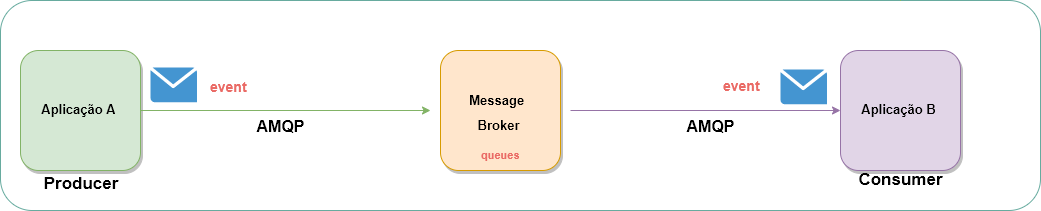
\includegraphics[width=0.9\linewidth]{Images/message_broker.png}
	\end{figure}


\end{frame}

\begin{frame}
	\frametitle{Mensageria}
	\framesubtitle{Nomenclatura}
	
	\begin{block}{AMQP - \textit{Advanced Message Queuing Protocol}}
		Protocolo de rede que permite a comunicação com um middleware (\textit{message broker}) para troca de mensagens assínconas. \\ \smallskip
		
		\begin{center}
			\textbf{Producer} $>$ \yellowbox{\textbf{Exchange} $>$ \textbf{Binding} $>$ \textbf{Queue}} $>$ \textbf{Consumer}
		\end{center}

		\begin{itemize}
			\item \textbf{Exchange}: é a porta de entrada das mensagens no \textit{message broker}.
			\item \textbf{Binding}: é o vínculo entre uma fila de mensagens e uma exchange. Regras de roteamento.
		\end{itemize}
	\end{block}

	\begin{figure}
		\centering
		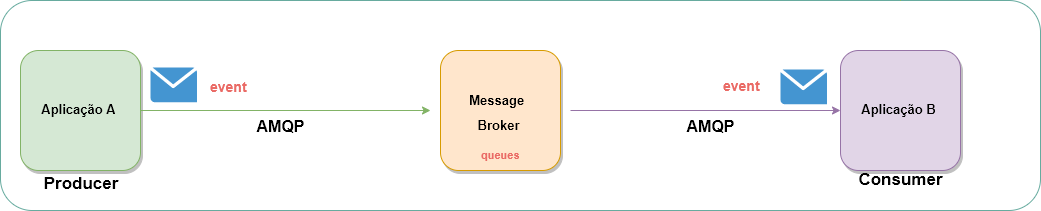
\includegraphics[width=0.9\linewidth]{Images/message_broker.png}
	\end{figure}


\end{frame}

\section{Material Complementar}

\begin{frame}
	\frametitle{Mensageria}
	\framesubtitle{Material Complementar}
	
	\begin{itemize}
		\item \iconLink{https://www.youtube.com/playlist?list=PLqONbZa3fPe4Z6sg7RQGaHlYqUjsliKAH}{\textbf{Playlist - Mensageria}}.\\Canal \textbf{Gabriel Faraday}.
		\item \iconLink{https://www.youtube.com/watch?v=A3gmE5yC97g}{\textbf{Apache Kafka e Spring Boot}}.\\Livro \textbf{Casa do Código}.
		\item \iconLink{https://www.casadocodigo.com.br/products/livro-apache-kafka}{\textbf{Aprendendo sobre mensageria}}.\\Canal \textbf{Daniele Leão}.
	\end{itemize}

\end{frame}

%------------------------------------------------

\section{Simulação}

\begin{frame}
	\frametitle{Mensageria}
	\framesubtitle{Simulação}
	\centering

	\begin{block}{Objetivo}
		Simular o envio de uma mensagem para uma fila de mensagens utilizando o RabbitMQ.
		\\ \bigskip
		\iconLink{https://tryrabbitmq.com/}{RabbitMQ Simulator Tool}
	\end{block}

\end{frame}

\section{Experimentos}

\begin{frame}
	\frametitle{Mensageria}
	\framesubtitle{Experimentos}

	{\Large \textbf{Experimento 1}} \\
	
	Acesse o repositório \href{https://github.com/rabbitmq/rabbitmq-tutorials?tab=readme-ov-file}{RabbitMQ Tutorials}, escolha uma linguagem de programação e realize os experimentos propostos.

	\begin{block}{Observações}
		\textbf{Pré-requisitos}: instalar o RabbitMQ.
	\end{block}

\end{frame}

% \begin{frame}
% 	\frametitle{Mensageria}
% 	\framesubtitle{Experimentos}

% 	\begin{block}{Experimento 2}
% 		Implementar um sistema básico de gestão de pedidos em um ambiente de comércio eletrônico utilizando RabbitMQ para facilitar a comunicação assíncrona entre diferentes partes do sistema.

% 		\begin{enumerate}
% 			\item O sistema deve consistir em pelo menos duas partes ou microserviços: um para o gerenciamento de pedidos e outro para o controle de estoque.
% 			\item Utilize RabbitMQ para a troca de mensagens entre os microserviços.
% 			\item Quando um pedido é feito, uma mensagem deve ser enviada para a fila do RabbitMQ indicando os detalhes do pedido.
% 			\item O microserviço de estoque deve consumir as mensagens da fila e atualizar o estoque conforme necessário.
% 			\item Considere a possibilidade de tratamento de mensagens de erro, como a falta de estoque para atender a um pedido.
% 		\end{enumerate}
		
% 	\end{block}

% \end{frame}
		
	
\end{document} 
